\section{Những thuật toán Heuristic giải quyết 2DCSP}
\subsection{Tạo Cột (Generate Column)}

\hspace{0.5cm}Bài toán cắt hai chiều (2DCSP) liên quan đến việc cắt nguyên liệu thành các mảnh nhỏ hơn để đáp ứng nhu cầu sản phẩm được chỉ định, đồng thời giảm thiểu lãng phí. Đây là một bài toán phức tạp về tổ hợp, đòi hỏi các chiến lược động để giải quyết hiệu quả các trường hợp quy mô lớn. Thuật toán được trình bày tạo mẫu cắt động và ưu tiên bố trí dựa trên kích thước sản phẩm và khả năng nguyên liệu sẵn có.

Thuật toán bao gồm các thành phần chính sau:

\textbf{Tạo mẫu động}

Thuật toán tạo các mẫu cắt động dựa trên kích thước và số lượng sản phẩm còn lại. Các sản phẩm được sắp xếp theo thứ tự giảm dần diện tích (\( \text{Width} \times \text{Height} \)) để ưu tiên các sản phẩm lớn hơn. Quá trình tạo mẫu điền lần lượt các mẫu bằng cách xem xét các vị trí khả thi cho từng sản phẩm.

Gọi \( P = \{p_1, p_2, \dots, p_n\} \) là tập hợp các sản phẩm, trong đó mỗi sản phẩm \( p_i \) có:
\[
\text{Kích thước}(p_i) = (w_i, l_i), \quad \text{Số lượng}(p_i) = d_i
\]

Các mẫu cắt được biểu diễn như sau:
\[
\text{Mẫu} = \{x_1, x_2, \dots, x_n\}, \quad x_i \text{ là số mảnh của } p_i \text{ trong mẫu}.
\]

Với mỗi sản phẩm \( p_i \), số lượng tối đa các mảnh có thể đặt trong nguyên liệu kích thước \( (W, H) \) là:
\[
\text{Số lượng tối đa}(p_i) = \min\left(q_i, \left\lfloor \frac{W}{w_i} \right\rfloor \times \left\lfloor \frac{H}{h_i} \right\rfloor\right).
\]

Để bố trí sản phẩm vào nguyên liệu, thuật toán xác định các vị trí khả thi bằng cách duyệt qua tất cả các tọa độ \( (x, y) \) trong nguyên liệu. Một vị trí là hợp lệ nếu sản phẩm không chồng lấn với các mảnh đã được đặt trước đó và nằm trong giới hạn kích thước của nguyên liệu.

Gọi \( S \) là nguyên liệu kích thước \( (W, H) \), và gọi \( p_i \) là sản phẩm kích thước \( (w_i, h_i) \). Một vị trí \( (x, y) \) là hợp lệ nếu:
\[
x + w_i \leq W, \quad y + h_i \leq H, \quad \text{và không chồng lấn với các mảnh đã đặt trước đó}.
\]

\textbf{Ưu tiên nguyên liệu}

Nguyên liệu được sắp xếp theo thứ tự giảm dần diện tích để ưu tiên các nguyên liệu lớn hơn cho việc bố trí:
\[
\text{Ưu tiên nguyên liệu} = \text{Diện tích}(S) = W \times H.
\]

\textbf{Quy trình thuật toán}

Quy trình được tóm tắt như sau:
\begin{enumerate}[1) ]
    \item Sắp xếp các sản phẩm theo diện tích giảm dần.

    \item Sắp xếp các nguyên liệu theo diện tích giảm dần.

    \item Tạo các mẫu cắt động cho nguyên liệu lớn nhất.

    \item Duyệt qua các mẫu để bố trí sản phẩm vào nguyên liệu:

    \begin{enumerate}
        \item Kiểm tra nếu tồn tại vị trí hợp lệ cho từng sản phẩm trong mẫu.
        \item Nếu tìm thấy vị trí, đặt sản phẩm và cập nhật việc sử dụng nguyên liệu.
    \end{enumerate}
   
    \item Nếu không tìm thấy vị trí hợp lệ, chuyển sang nguyên liệu tiếp theo.

    \item Lặp lại cho đến khi tất cả nhu cầu sản phẩm được đáp ứng hoặc nguyên liệu đã hết.
\end{enumerate}

\begin{figure}[!htp]
    \centering
    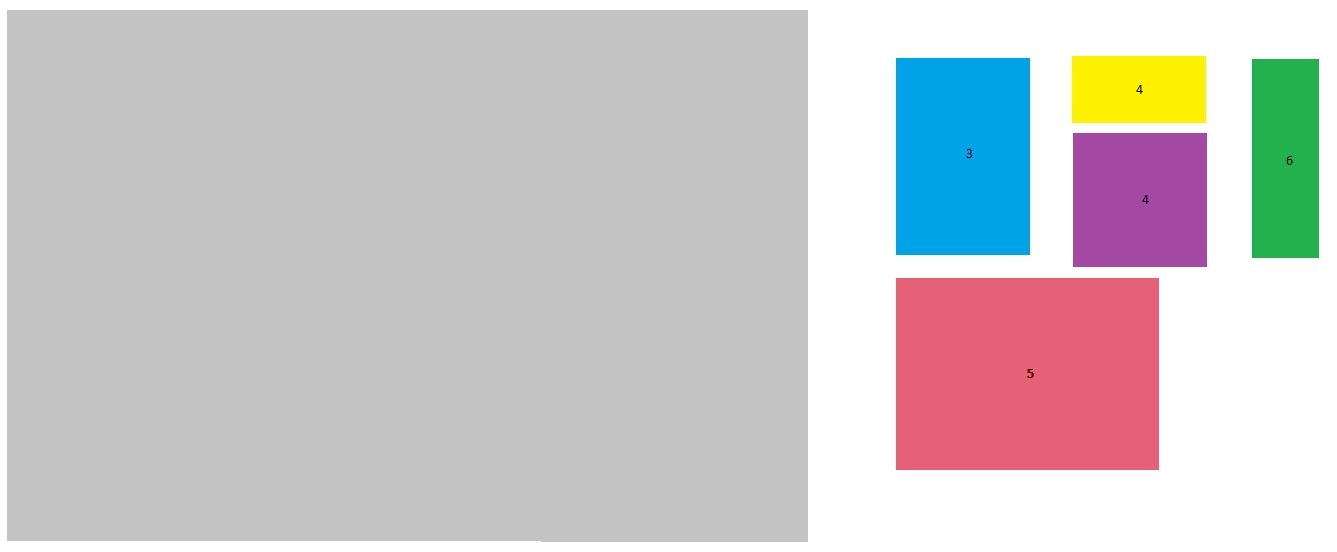
\includegraphics[width=0.5\linewidth]{Images/gencolumn.png}
    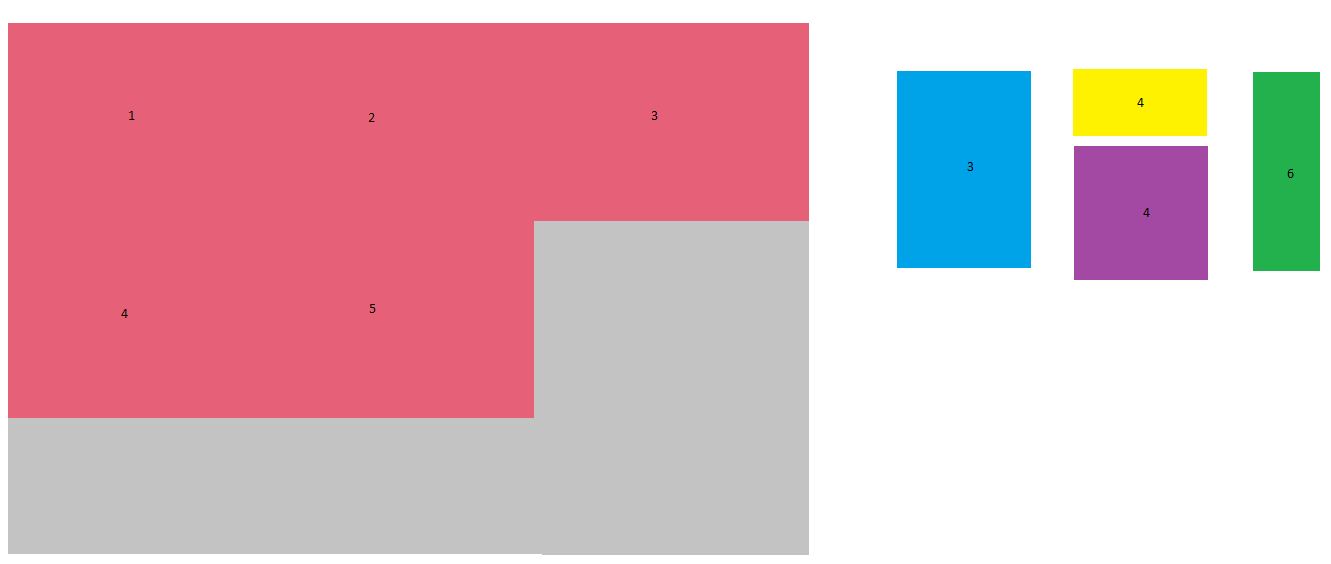
\includegraphics[width=0.5\linewidth]{Images/gencolumn_res.png}
    \caption{Bố trí một nguyên liệu sau khi áp dụng thuật toán Generate Column.}
    \label{fig:stock-layout}
\end{figure}

\subsection{Phân bổ Best-Fit với Lựa chọn Heuristic}

\hspace{0.5cm}\textbf{Thuật toán Best-Fit} là một giải pháp tối ưu cho việc sắp xếp sản phẩm lên các vật liệu tồn kho, được thiết kế tỉ mỉ nhằm giảm thiểu lãng phí và tối đa hóa hiệu suất sử dụng. Bằng cách kết hợp các quyết định lặp lại với cơ chế chấm điểm tiên tiến, thuật toán xác định cách bố trí hiệu quả nhất cho từng sản phẩm. Phần này sẽ trình bày nguyên tắc cơ bản, quy trình hoạt động, và các ưu điểm của thuật toán trong thực tế.

\vspace{0.3cm}
\noindent\textbf{Nguyên tắc cơ bản}

Thuật toán dựa trên \textit{chiến lược đặt sản phẩm theo đường bao (skyline-based placement strategy)} để xác định vị trí tối ưu cho từng sản phẩm, với các tiêu chí sau:
\begin{enumerate}
    \item \textbf{Hiệu suất sử dụng diện tích:} Ưu tiên sắp xếp các sản phẩm sao cho giảm thiểu không gian chưa sử dụng.
    \item \textbf{Căn chỉnh chiều cao:} Đảm bảo các sản phẩm được sắp xếp theo chiều dọc để tạo sự gọn gàng.
    \item \textbf{Ưu tiên căn chỉnh theo cạnh:} Khuyến khích sắp xếp sản phẩm dọc theo các cạnh của vật liệu để giảm sự phân mảnh.
    \item \textbf{Theo dõi hiệu suất sử dụng:} Giám sát tỷ lệ diện tích đã sử dụng để tối ưu hóa hiệu suất vật liệu.
\end{enumerate}

\vspace{0.3cm}
\noindent\textbf{Quy trình hoạt động}

Thuật toán Best-Fit hoạt động theo các bước sau:

\begin{enumerate}[1) ]
    \item \textbf{Khởi tạo:} Thiết lập các cấu trúc dữ liệu để theo dõi:
    \begin{itemize}
        \item \textbf{Hiệu suất sử dụng từng vật liệu:} Tỷ lệ phần trăm diện tích đã sử dụng.
        \item \textbf{Các vị trí đã chiếm:} Các tọa độ trong vật liệu đã được sử dụng.
        \item \textbf{Các tham số:} Như ngưỡng lãng phí và tỷ lệ chiều cao tối đa.
    \end{itemize}
    \item \textbf{Tính toán đường bao (Skyline):} Xây dựng hồ sơ đường bao cho mỗi vật liệu:
    \[
    \text{Skyline}[i] = \max(\text{tọa độ y được chiếm tại } x = i)
    \]
    \begin{figure}[!htp]
        \centering
        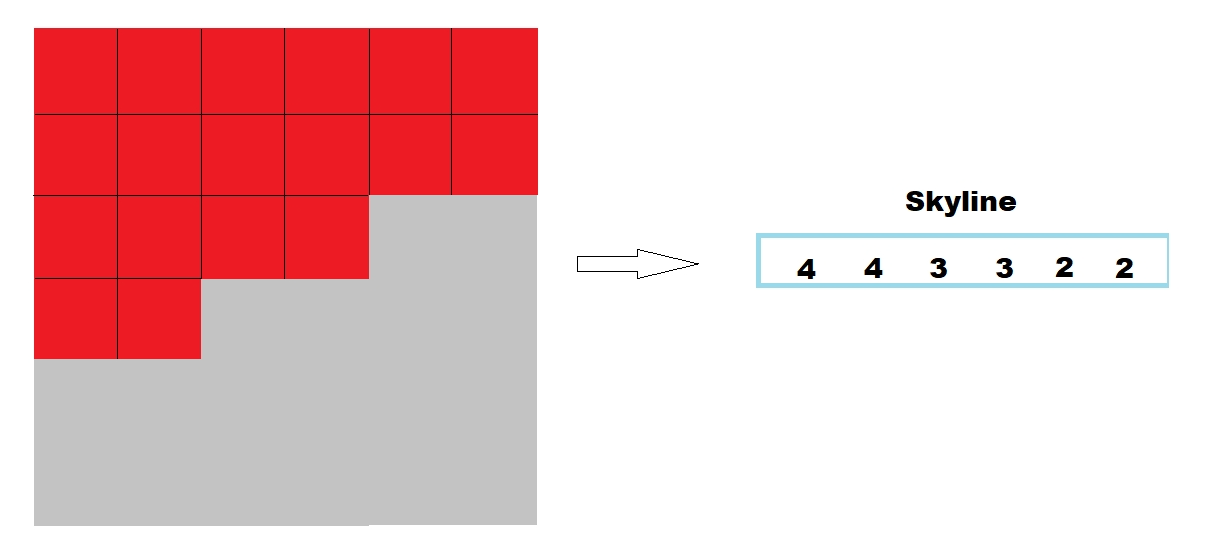
\includegraphics[width=0.4\linewidth]{Images/skyline.png}
        \caption{Hồ sơ đường bao của một vật liệu đã sử dụng}
        \label{fig:enter-label}
    \end{figure}
    Hồ sơ này giúp xác định không gian theo chiều dọc còn trống tại mỗi vị trí ngang.
    \item \textbf{Chiến lược đặt sản phẩm:} 
    \begin{enumerate}[a)]
        \item Sắp xếp các sản phẩm theo thứ tự giảm dần của diện tích (\( \text{Width} \times \text{Height} \)).
        \item Với mỗi sản phẩm, đánh giá các vị trí khả thi dựa trên hồ sơ đường bao.
        \item Gán điểm số cho từng vị trí dựa trên:
        \begin{itemize}
            \item \textit{Lãng phí diện tích:} Không gian không sử dụng xung quanh sản phẩm.
            \item \textit{Phạt chiều cao:} Sự không đều về chiều cao so với đường bao hiện tại.
            \item \textit{Thưởng căn chỉnh cạnh:} Khuyến khích căn chỉnh sản phẩm theo các cạnh của vật liệu.
            \item \textit{Thưởng hiệu suất sử dụng:} Điểm cao hơn cho việc tối đa hóa không gian được lấp đầy.
        \end{itemize}
        \item Chọn vị trí có điểm số lãng phí thấp nhất.
    \end{enumerate}
    \item \textbf{Cập nhật trạng thái:} Sau khi đặt sản phẩm:
    \begin{itemize}
        \item Cập nhật các vị trí đã chiếm và hồ sơ đường bao của vật liệu.
        \item Điều chỉnh thống kê hiệu suất sử dụng của vật liệu.
    \end{itemize}
    \item \textbf{Kết thúc:} Lặp lại cho đến khi tất cả sản phẩm được đặt hoặc không còn vị trí khả thi.
\end{enumerate}

\vspace{0.3cm}
\noindent\textbf{Tính toán lãng phí}

Thuật toán tính \textbf{điểm số lãng phí} để đánh giá các vị trí khả thi:
\[
\text{Điểm số lãng phí} = 
\]
\[
(1 - \text{Hiệu suất sử dụng diện tích}) + \text{Phạt chiều cao} - \text{Thưởng căn chỉnh cạnh} - \text{Thưởng hiệu suất sử dụng}
\]
Điểm số này cân bằng nhiều yếu tố để xác định vị trí sắp xếp hiệu quả nhất.

\vspace{0.3cm}
\noindent\textbf{Ưu điểm của thuật toán Best-Fit}
\begin{itemize}
    \item \textbf{Chiến lược thích ứng:} Linh hoạt điều chỉnh vị trí đặt dựa trên hồ sơ vật liệu.
    \item \textbf{Hiệu quả vật liệu:} Giảm thiểu lãng phí và đạt tỷ lệ sử dụng cao.
    \item \textbf{Khả năng mở rộng:} Xử lý hiệu quả số lượng lớn sản phẩm và kích thước vật liệu đa dạng.
\end{itemize}

Bằng cách tích hợp liền mạch các phương pháp đường bao với hệ thống chấm điểm tiên tiến, thuật toán Best-Fit cung cấp một giải pháp mạnh mẽ và mở rộng để giải quyết bài toán sắp xếp sản phẩm, đảm bảo tối ưu hóa sử dụng vật liệu và giảm thiểu lãng phí.